\section{Assembling Paired-end Reads}

The use of paired-end data in \textit{de novo} genome assembly results in better
quality assemblies, particularly for larger, more complex genomes. In addition,
paired-end constraint violation (expected distance and orientation of paired
reads) can be used to identify misassemblies.

\begin{warning}
If you are doing \textit{de novo} assembly, pay the extra and get paired-ends:
they're worth it!
\end{warning}

\begin{note}
The data you will examine in this exercise is again from Staphylococcus aureus
which has a genome of around 3MBases. The reads are Illumina paired end with an
insert size of $~$350 bp.

The required data can be downloaded from the SRA. Specifically, the run data
(SRR022852) from the SRA Sample SRS004748.

\center{\url{http://www.ebi.ac.uk/ena/data/view/SRS004748}}

\end{note}

\begin{information}
The following exercise focuses on preparing the paired-end FASTQ files ready for
Velvet, using Velvet in paired-end mode and comparing results with Velvet's
'auto' option.
\end{information}

\begin{steps}
First move to the directory you made for this exercise and make a suitable named
directory for the exercise:
\begin{lstlisting}
cd ~/NGS/velvet/part2 
mkdir SRS004748 
cd SRS004748
\end{lstlisting}

There is no need to download the read files, as they are already stored
locally. You will simply create a symlink to this pre-downloaded data using
the following commands:
\begin{lstlisting}
ln -s ~/NGS/Data/SRR022852_?.fastq.gz ./
\end{lstlisting}

It is interesting to monitor the computer's resource utilisation, particularly
memory. A simple way to do this is to open a second terminal and in it type:
\begin{lstlisting}
top
\end{lstlisting}
\end{steps}

\begin{note}
\texttt{top} is a program that continually monitors all the processes running on
your computer, showing the resources used by each. Leave this running and refer
to it periodically throughout your Velvet analyses. Particularly if they are
taking a long time or whenever your curiosity gets the better of you. You should
find that as this practical progresses, memory usage will increase
significantly.

Now, back to the first terminal, you are ready to run \texttt{velveth} and
\texttt{velvetg}. The reads are \texttt{-shortPaired} and for the
first run you should not use any parameters for \texttt{velvetg}.
\end{note}

\begin{information}
From this point on, where it will be informative to time
your runs. This is very easy to do, just prefix the command to run the program
with the command \texttt{time}. This will cause UNIX to report how long the program took
to complete its task.
\end{information}

\begin{steps}
Set the two stages of velvet running, whilst you watch the memory usage as
reported by \texttt{top}. Time the \texttt{velvetg} stage:
\begin{lstlisting}
velveth run_25 25 -fmtAuto -create_binary -shortPaired -separate SRR022852_1.fastq.gz SRR022852_2.fastq.gz
time velvetg run_25
\end{lstlisting}

\end{steps}

\begin{questions}
What does \texttt{-fmtAuto} and \texttt{-create\_binary} do? (see help menu)
\begin{answer}
\texttt{-fmtAuto} tries to detect the correct format of the input files e.g.
  FASTA, FASTQ and whether they are compressed or not.

\texttt{-create\_binary} outputs sequences as a binary file. That means that
  \texttt{velvetg} can read the sequences from the binary file more quickly that
  from the original sequence files.
\end{answer}

Comment on the use of memory and CPU for \texttt{velveth} and \texttt{velvetg}?
\begin{answer}
\texttt{velveth} uses only one CPU while \texttt{velvetg} uses all possible CPUs
for some parts of the calculation.
\end{answer}
 
How long did \texttt{velvetg} take?
\begin{answer}
My own measurements are:\\
\texttt{real    1m8.877s; user    4m15.324s; sys     0m4.716s}
\end{answer}

\end{questions}

\begin{steps}
Next, after saving your \texttt{contigs.fa} file from being overwritten, set the
cut-off parameters that you investigated in the previous exercise and rerun
\texttt{velvetg}.
time and monitor the use of resources as previously. Start with
\texttt{-cov\_cutoff 16} thus:
\begin{lstlisting}
mv run_25/contigs.fa run_25/contigs.fa.0
time velvetg run_25 -cov_cutoff 16
\end{lstlisting}

Up until now, \texttt{velvetg} has ignored the paired-end information. Now try
running \texttt{velvetg} with both \texttt{-cov\_cutoff 16} and
\texttt{-exp\_cov 26}, but first save your \texttt{contigs.fa} file. By using
\texttt{-cov\_cutoff} and \texttt{-exp\_cov}, \texttt{velvetg} tries to estimate
the insert length, which you will see in the \texttt{velvetg} output. The
command is, of course:
\begin{lstlisting}
mv run_25/contigs.fa run_25/contigs.fa.1
time velvetg run_25 -cov_cutoff 16 -exp_cov 26
\end{lstlisting}

\end{steps}

\begin{questions}
Comment on the time required, use of memory and CPU for \texttt{velvetg}?
\begin{answer}
Runtime is lower when velvet can reuse previously calculated data. By using
\texttt{-exp\_cov}, the memory usage increases.
\end{answer}

Which insert length does Velvet estimate?
\begin{answer}
Paired-end library 1 has length: 228, sample standard deviation: 26
\end{answer}

\end{questions}

\begin{steps}
Next try running \texttt{velvetg} in `paired-end mode`. This entails running \texttt{velvetg}
specifying the insert length with the parameter \texttt{-ins\_length} set to 350. Even
though velvet estimates the insert length it is always advisable to check /
provide the insert length manually as velvet can get the statistics wrong due
to noise. Just in case, save your last version of \texttt{contigs.fa}. The commands are:
\begin{lstlisting}
mv run_25/contigs.fa run_25/contigs.fa.2
time velvetg run_25 -cov_cutoff 16 -exp_cov 26 -ins_length 350
mv run_25/contigs.fa run_25/contigs.fa.3
\end{lstlisting}
\end{steps}

\begin{questions}
How fast was this run?
\begin{answer}
My own measurements are:\\
\texttt{real    0m29.792s; user    1m4.372s; sys     0m3.880s}
\end{answer}

\end{questions}

\begin{steps}
Take a look into the Log file.
\end{steps}

\begin{questions}
What is the N50 value for the \texttt{velvetg} runs using the switches:\\
\begin{answer}
Base run: 19,510 bp
\end{answer}
\texttt{-cov\_cutoff 16}
\begin{answer}
24,739 bp
\end{answer}

\texttt{-cov\_cutoff 16 -exp\_cov 26}
\begin{answer}
61,793 bp
\end{answer}

\texttt{-cov\_cutoff 16 -exp\_cov 26 -ins\_length 350}
\begin{answer}
n50 of 62,740 bp; max 194,649 bp; total 2,871,093 bp
\end{answer}

\end{questions}

\begin{steps}
Try giving the \texttt{-cov\_cutoff} and/or \texttt{-exp\_cov} parameters the
value \texttt{auto}. See the \texttt{velvetg} help to show you how. The
information Velvet prints during running includes information about the values
used (coverage cut-off or insert length) when using the \texttt{auto} option.
\end{steps}

\begin{questions}
What coverage values does Velvet choose (hint: look at the output that Velvet
produces while running)?
\begin{answer}
Median coverage depth = 26.021837\\
Removing contigs with coverage $<$ 13.010918 \ldots
\end{answer}

How does the N50 value change?
\begin{answer}
n50 of 68,843 bp; max 194,645 bp; total 2,872,678 bp
\end{answer}
\end{questions}

\begin{steps}
Run \texttt{gnx} on all the \texttt{contig.fa} files you have generated in the
course of this exercise. The command will be:
\begin{lstlisting}
gnx -min 100 -nx 25,50,75 run_25/contigs.fa*
\end{lstlisting}
\end{steps}

\begin{questions}
For which runs are there Ns in the \texttt{contigs.fa} file and why? 
\begin{answer}
contigs.fa.2, contigs.fa.3, contigs.fa\\
Velvet tries to use the provided (or infers) the insert length and fills
ambiguous regions with Ns.
\end{answer}

Comment on the number of contigs and total length generated for each run.
\begin{answer}
\begin{table}[H]
  %\centering
    \begin{tabular}{ll}
    \toprule
    Filename & \# contigs & Total length & \# Ns \\
    \midrule
    Contigs.fa.0 & 631 & 2,830,659 & 0 \\
    Contigs.fa.1 & 580 & 2,832,670 & 0 \\
    Contigs.fa.2 & 166 & 2,849,919 & 4,847 \\
    Contigs.fa.3 & 166 & 2,856,795 & 11,713 \\
    Contigs.fa & 163 & 2,857,439 & 11,526 \\
    \bottomrule
    \end{tabular}%
  \caption{\label{tab:velvetrunresults}}%
\end{table}%
\end{answer}
\end{questions}

\subsection{AMOS Hawkeye}

We will now output the assembly in the AMOS massage format and visualise the
assembly using AMOS Hawkeye.

\begin{steps}
Run \texttt{velvetg} with appropriate arguments and output the AMOS message
file, then convert it to an AMOS bank and open it in Hawkeye:
\begin{lstlisting}
time velvetg run_25 -cov_cutoff 16 -exp_cov 26 -ins_length 350 -amos_file yes -read_trkg yes 
time bank-transact -c -b run_25/velvet_asm.bnk -m run_25/velvet_asm.afg         
hawkeye run_25/velvet_asm.bnk
\end{lstlisting}
\end{steps}

\begin{questions}
Looking at the scaffold view of a contig, comment on the proportion of ``happy
mates'' to ``compressed mates'' and ``stretched mates''.
\begin{answer}
Nearly all mates are compressed with no stretched mates and very few happy
mates.
\end{answer}

What is the mean and standard deviation of the insert size reported under the
Libraries tab?
\begin{answer}
Mean: 350 bp
SD: 35 bp
\end{answer}

Look at the actual distribution of insert sizes for this library. Can you
explain where there is a difference between the mean and SD reported in those
two places?
\begin{answer}
We specified \texttt{-ins\_length 350} to the \texttt{velvetg} command. Velvet
uses this value, in the AMOS message file that it outputs, rather than its own
estimate.
\end{answer}
\end{questions}

\begin{steps}
You can get AMOS to re-estimate the mean and SD of insert sizes using
intra-contig pairs. First, close Hawkeye and then run the following commands
before reopening the AMOS bank to see what has changed.
\begin{lstlisting}
asmQC -b run_25/velvet_asm.bnk -scaff -recompute -update -numsd 2
hawkeye run_25/velvet_asm.bnk
\end{lstlisting}
\end{steps}

\begin{questions}
Looking at the scaffold view of a contig, comment on the proportion of ``happy
mates'' to ``compressed mates'' and ``stretched mates''.
\begin{answer}
There are only a few compressed and stretched mates compared to happy mates.
There are similar numbers of stretched and compressed mates.
\end{answer}

What is the mean and standard deviation of the insert size reported under the
Libraries tab?
\begin{answer}
TODO
Mean: 226 bp
SD: 25 bp
\end{answer}

Look at the actual distribution of insert sizes for this library. Does the mean
and SD reported in both places now match?
\begin{answer}
Yes
\end{answer}

Can you find a region with an unusually high proportion of stretched, compressed,
incorrectly orientated or linking mates? What might this situation indicate?
\begin{answer}
This would indicate a possible misassembly and worthy of further investigation.

Look at the largest scaffold, there are stacks of stretched pairs which span
contig boundaries. This indicates that the gap size has been underestimated
during the scaffolding phase.
\end{answer}
\end{questions}


\subsection{Velvet and Data Quality}
So far we have used the raw read data without performing any quality control or
read trimming prior to doing our velvet assemblies.

\begin{warning}
Velvet does not use quality information present in FASTQ files.
\end{warning}

For this reason, it is vitally important to perform read QC and quality
trimming. In doing so, we remove errors/noise from the dataset which in turn
means velvet will run faster, will use less memory and will produce a better
assembly. Assuming we haven't compromised too much on coverage.

\begin{information}
To investigate the effect of data quality, we will use the run data (SRR023408)
from the SRA experiment SRX008042. The reads are Illumina paired end with an
insert size of 92 bp.
\end{information}

\begin{steps}
Go back to the main directory for this exercise and create and enter a new
directory dedicated to this phase of the exercise. The commands are:
\begin{lstlisting}
cd ~/NGS/velvet/part2 
mkdir SRX008042 
cd SRX008042
\end{lstlisting}

Create symlinks to the read data files that we downloaded for you from the SRA:
\begin{lstlisting}
ln -s ~/NGS/Data/SRR023408_?.fastq.gz ./
\end{lstlisting}
\end{steps}

\begin{note}
We will use FastQC, a tool you should be familiar with, to visualise the quality
of our data. We will use FastQC in the Graphical User Interface (GUI) mode.
\end{note}

\begin{steps}
Start FastQC and set the process running in the background, by using a trailing
\texttt{\&}, so we get control of our terminal back for entering more commands:
\begin{lstlisting}
fastqc &
\end{lstlisting}
\end{steps}

\begin{steps}
Open the two compressed FASTQ files (File $->$ Open) by selecting them both and clicking OK).
Look at tabs for both files:
\end{steps}

\begin{figure}[H]
\centering
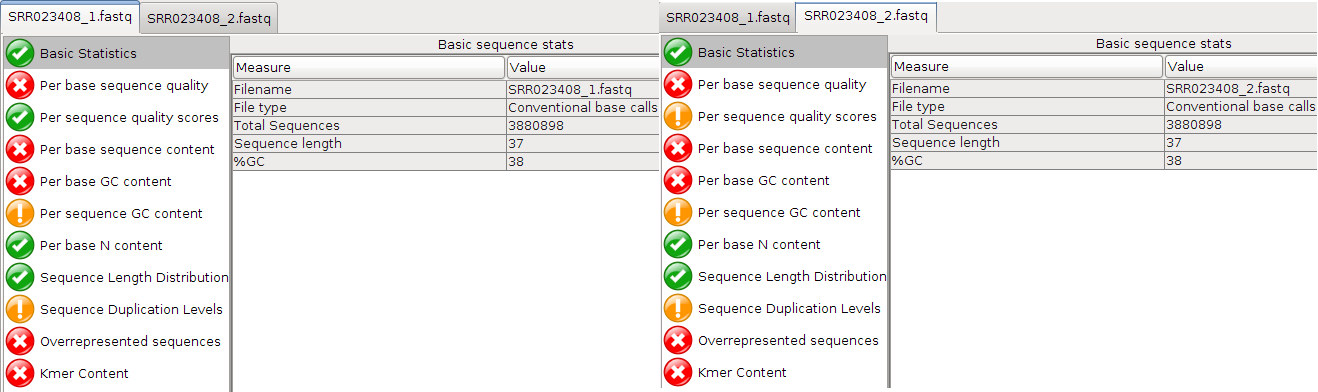
\includegraphics[width=0.8\textwidth]{de_novo/velvet/paired_fastqc.png}
\caption{\label{fig:paired_fastqc}}
\end{figure}

\begin{questions}
Are the quality scores the same for both files?
\begin{answer}
Overall yes
\end{answer}

Which value varies?
\begin{answer}
Per sequence quality scores
\end{answer}

Take a look at the Per base sequence quality for both files. Did you note that
it is not good for either file?
\begin{answer}
The quality score of both files drop very fast. Qualities of the REV strand drop
faster than the FWD strand. This is because the template has been sat around
while the FWD strand was sequenced.
\end{answer}

At which positions would you cut the reads if we did ``fixed length trimming''?
\begin{answer}
Looking at the ``Per base quality" and ``Per base sequence content'', I would
choose around 27
\end{answer}

Why does the quality deteriorate towards the end of the read?
\begin{answer}
Errors more likely for later cycles
\end{answer}

Does it make sense to trim the 5' start of reads?
\begin{answer}
Looking at the ``Per base sequence content", yes - there is a clear signal at the beginning.
\end{answer}
\end{questions}

\begin{steps}
Have a look at the other options that FastQC offers.
\end{steps}

\begin{questions}
Which other statistics could you use to support your trimming strategy?
\begin{answer}
``Per base sequence content", ``Per base GC content", ``Kmer content", ``Per
base sequence quality"
\end{answer}
\end{questions}

\begin{figure}[H]
\centering
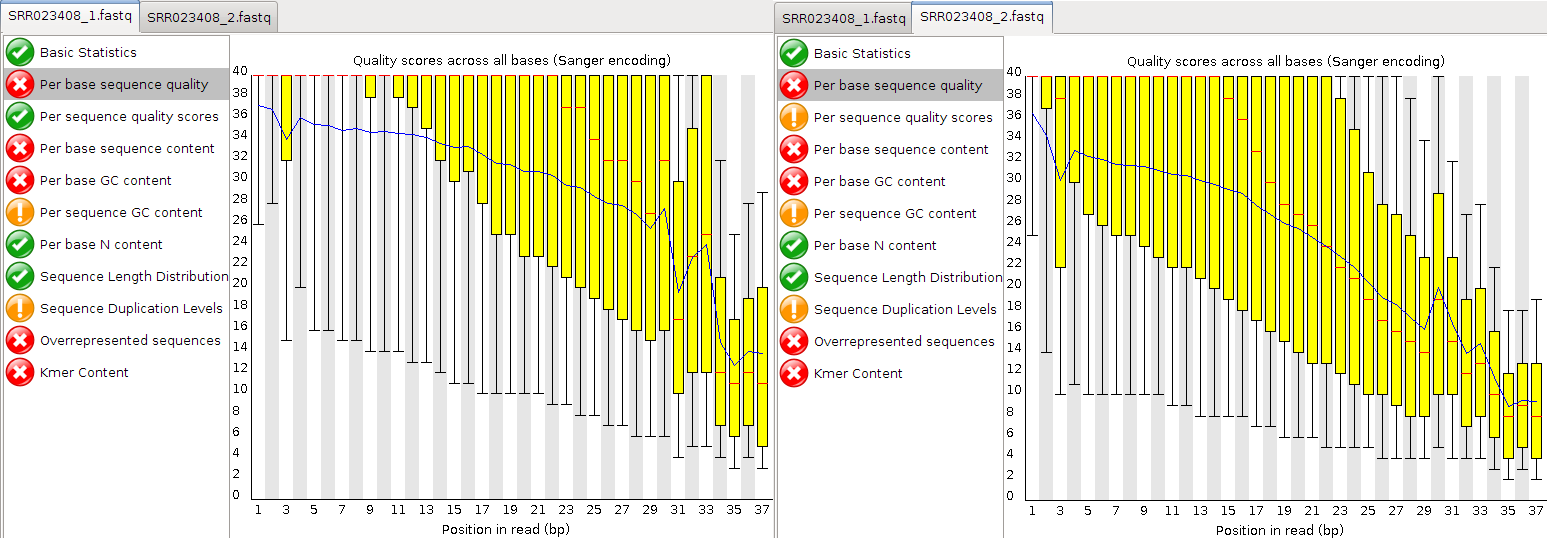
\includegraphics[width=0.8\textwidth]{de_novo/velvet/paired_fastqc_quality_plots.png}
\caption{\label{fig:paired_fastqc_quality_plots}}
\end{figure}

\begin{steps}
Once you have decided what your trim points will be, close FastQC.
We will use \texttt{fastx\_trimmer} from the FASTX-Toolkit to perform
fixed-length trimming. For usage information see the help:
\begin{lstlisting}
fastx_trimmer -h
\end{lstlisting}

\begin{note}
\texttt{fastx\_trimmer} is not able to read compressed FASTQ files, so we first
need to decompress the files ready for input.
\end{note}

The suggestion (hopefully not far from your own thoughts?) is that you trim your
reads as follows:

\begin{lstlisting}
gunzip < SRR023408_1.fastq.gz > SRR023408_1.fastq
gunzip < SRR023408_2.fastq.gz > SRR023408_2.fastq
fastx_trimmer -Q 33 -f 4 -l 32 -i SRR023408_1.fastq -o SRR023408_trim1.fastq 
fastx_trimmer -Q 33 -f 3 -l 29 -i SRR023408_2.fastq -o SRR023408_trim2.fastq
\end{lstlisting}

\begin{advanced}
Many NGS read files are large. This means that simply reading and writing files
can become the bottleneck, also known as I/O bound. Therefore, it is often good practice to
avoid unnecessary disk read/write.

We could do what is called pipelining to send a stream of data from one command
to another, using the pipe (\texttt{|}) character, without the need for
intermediary files. The following command would achieve this:
\begin{lstlisting}
gunzip --to-stdout < SRR023408_1.fastq.gz | fastx_trimmer -Q 33 -f 4 -l 32 -o SRR023408_trim1.fastq 
gunzip --to-stdout < SRR023408_2.fastq.gz | fastx_trimmer -Q 33 -f 3 -l 29 -o SRR023408_trim2.fastq
\end{lstlisting}
\end{advanced}

Now run \texttt{velveth} with a k-mer value of 21 for both the untrimmed and
trimmed read files in \texttt{-shortPaired} mode. Separate the output of the two
executions of \texttt{velveth} into suitably named directories, followed by
\texttt{velvetg}:
\begin{lstlisting}
# untrimmed reads
velveth run_21 21 -fmtAuto -create_binary -shortPaired -separate SRR023408_1.fastq SRR023408_2.fastq
time velvetg run_21

# trimmed reads
velveth run_21trim 21 -fmtAuto -create_binary -shortPaired -separate SRR023408_trim1.fastq SRR023408_trim2.fastq
time velvetg run_21trim
\end{lstlisting}
\end{steps}

\begin{questions}
How long did the two \texttt{velvetg} runs take?
\begin{answer}
run\_25:      \texttt{real    3m16.132s; user    8m18.261s; sys     0m7.317s}\\
run\_25trim:  \texttt{real    1m18.611s; user    3m53.140s; sys     0m4.962s}
\end{answer}

What N50 scores did you achieve?
\begin{answer}
Untrimmed: 11\\
Trimmed: 15
\end{answer}

What were the overall effects of trimming?
\begin{answer}
Time saving, increased N50, reduced coverage
\end{answer}
\end{questions}

\begin{steps}
The evidence is that trimming improved the assembly. The thing to do surely, is
to run \texttt{velvetg} with the \texttt{-cov\_cutoff} and \texttt{-exp\_cov}. In order
to use \texttt{-cov\_cutoff} and \texttt{-exp\_cov} sensibly, you need to
investigate with R, as you did in the previous exercise, what parameter values
to use. Start up R and produce the weighted histograms:
\begin{lstlisting}[style=R]
R --no-save
library(plotrix) 
data <- read.table("run_21/stats.txt", header=TRUE) 
data2 <- read.table("run_21trim/stats.txt", header=TRUE) 
par(mfrow=c(1,2))
weighted.hist(data$short1_cov, data$lgth, breaks=0:50)
weighted.hist(data2$short1_cov, data2$lgth, breaks=0:50)
\end{lstlisting}

\begin{figure}[H]
\centering
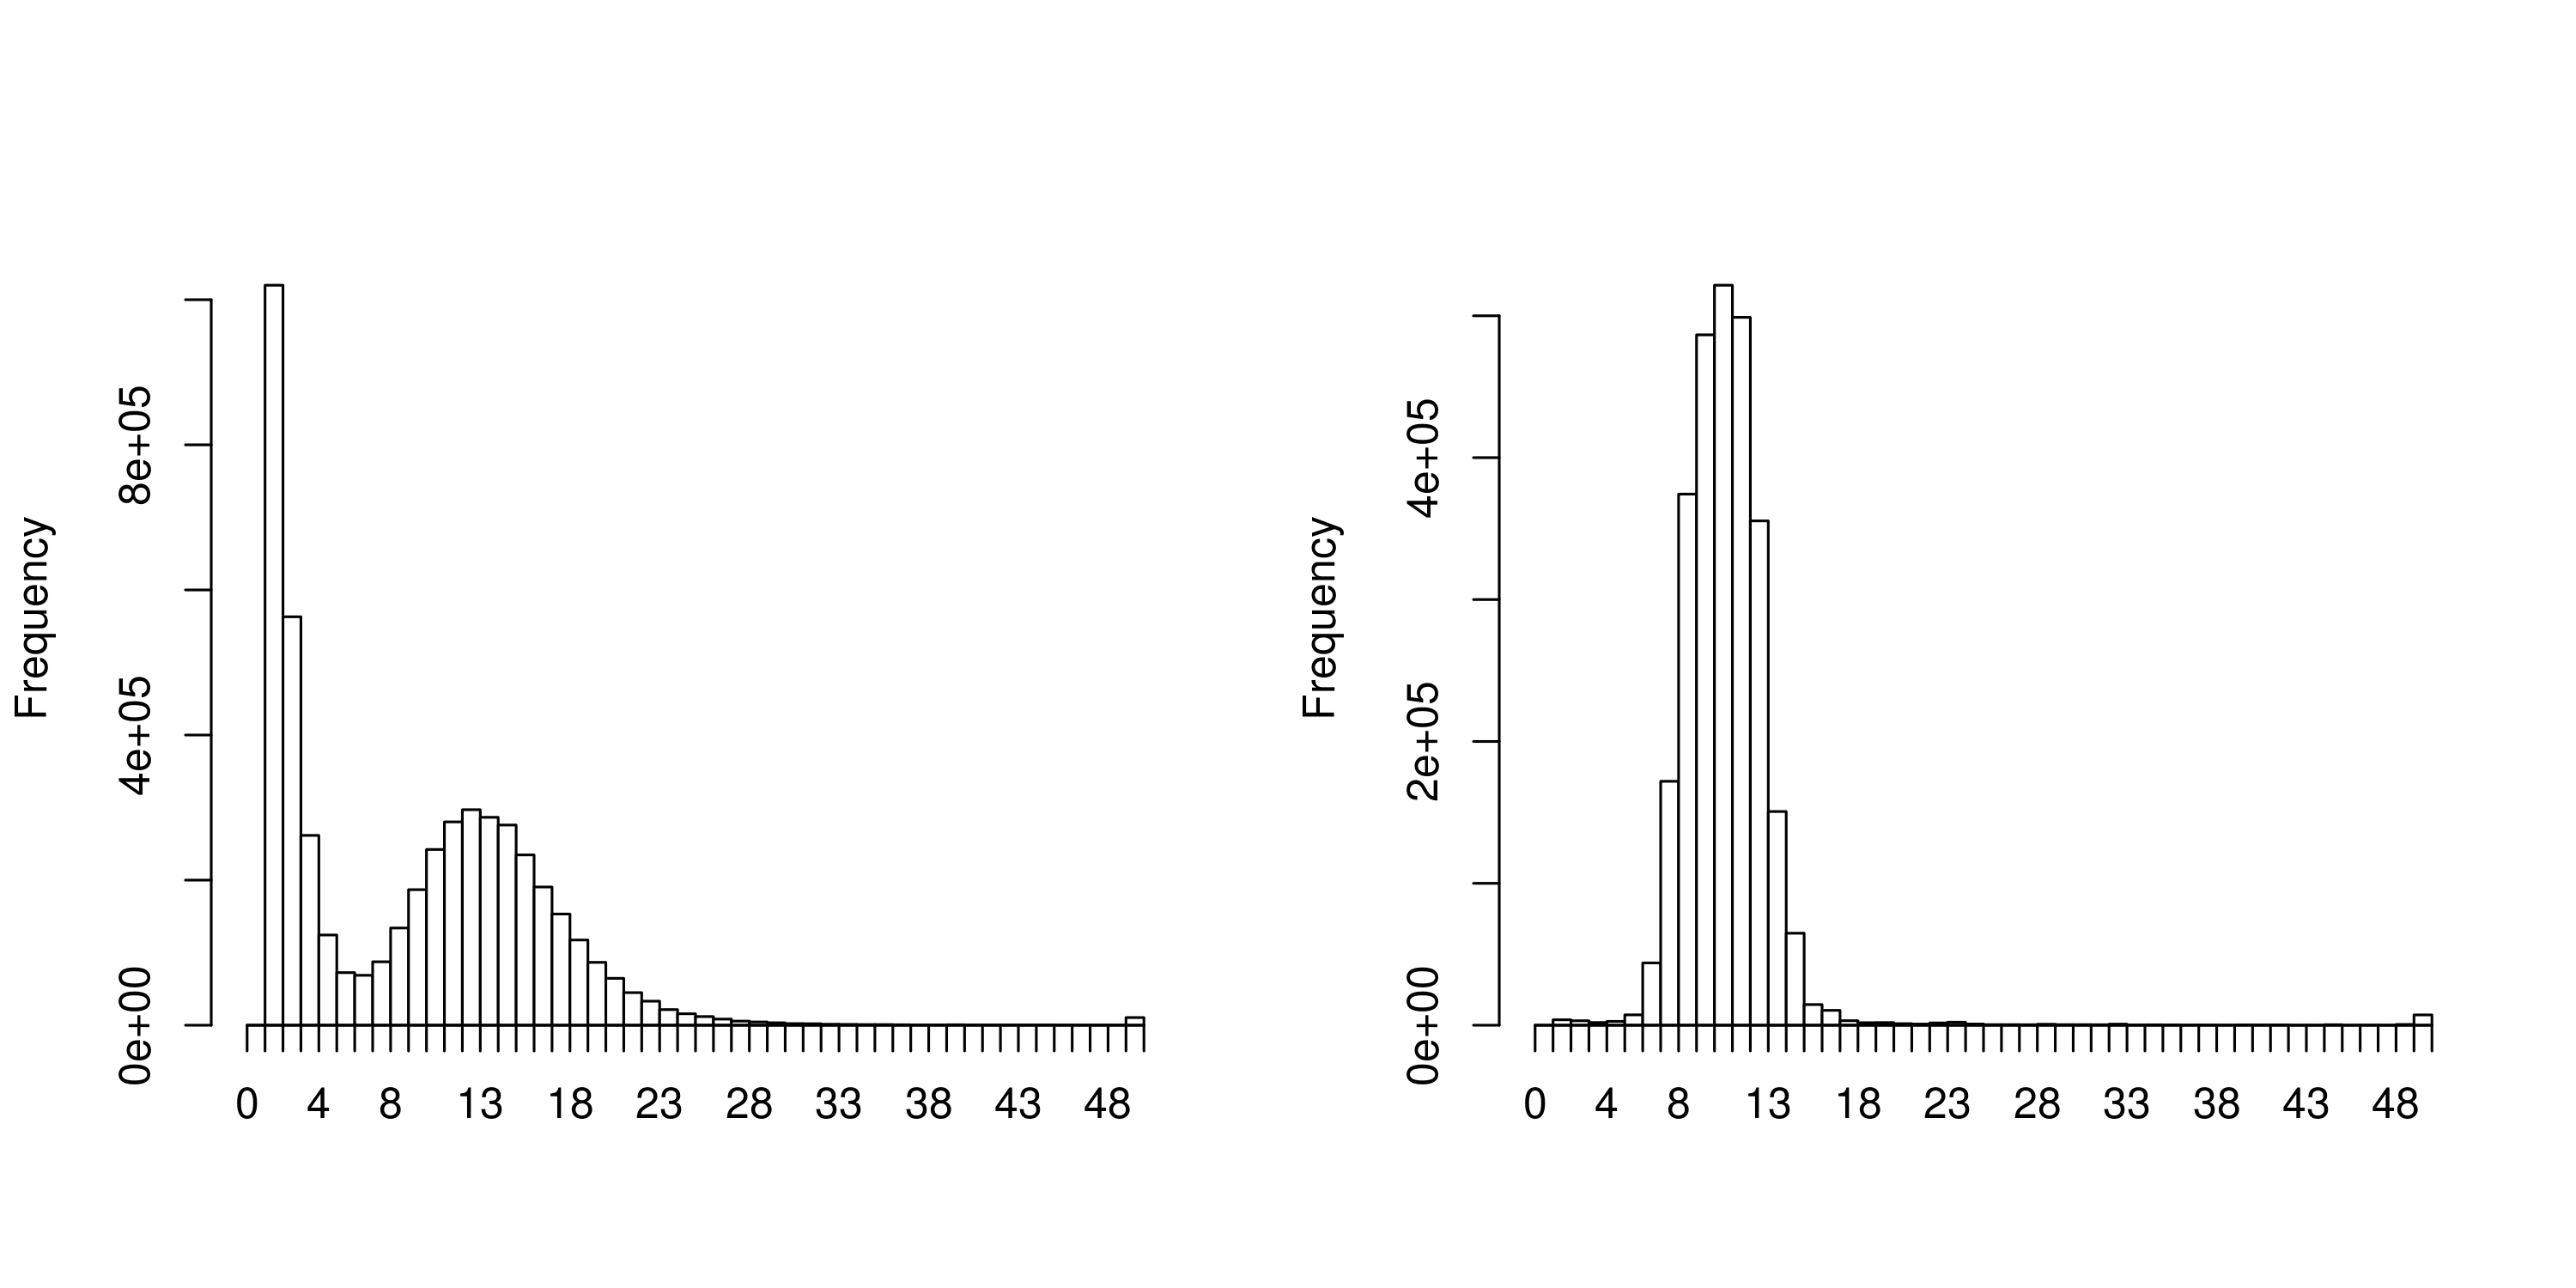
\includegraphics[width=0.8\textwidth]{de_novo/velvet/velvet_Rplot002.png}
\caption{\label{fig:velvet_Rplot002} Weighted k-mer coverage histograms of the paired-end reads pre-trimmed (left) and post-trimmed (right).}
\end{figure}

For the untrimmed read histogram (left) there is an expected coverage of around
13 with a coverage cut-off of around 7. For the trimmed read histogram (right)
there is an expected coverage of around 9 with a coverage cut-off of around 5.

If you disagree, feel free to try different settings, but first quit R before
running \texttt{velvetg}:
\begin{lstlisting}[style=R]
q()
\end{lstlisting}

\begin{lstlisting}
time velvetg run_21 -cov_cutoff 7 -exp_cov 13 -ins_length 92
time velvetg run_21trim -cov_cutoff 5 -exp_cov 9 -ins_length 92
\end{lstlisting}

\end{steps}

\begin{questions}
How good does it look now?\\
\begin{answer}
Still not great
\end{answer}
Comment on:\\ 
Runtime
\begin{answer}
Reduced runtime
\end{answer}

Memory
\begin{answer}
Lower memory usage
\end{answer}

k-mer choice (Can you use k-mer 31 for a read of length 30 bp?)
\begin{answer}
K-mer has to be lower than the read length and the K-mer coverage should be
sufficient to produce results.
\end{answer}

Does less data mean ``worse" results?
\begin{answer}
Not necessarily. If you have lots of data you can safely remove poor data
without too much impact on overall coverage.
\end{answer}
  
How would a smaller/larger k-mer size behave?
\begin{answer}
% TODO
\end{answer}
\end{questions}

\begin{steps}
Compare the results, produced during the last exercises, with each other:

\begin{table}[H]
  \centering
    \begin{tabular*}{0.9\textwidth}{l|l|l|l}
    \toprule
    Metric & SRR022852 & SRR023408 & SRR023408.trimmed \\
    \midrule
    Overall Quality (1-5) & & & \\[0.5\questionspacing]
    \hline
    bp Coverage & & & \\[0.5\questionspacing]
    \hline
    k-mer Coverage & & & \\[0.5\questionspacing]
    \hline
    N50 (k-mer used) & & & \\[0.5\questionspacing]
    \bottomrule
    \end{tabular*}
  \caption{\label{tab:comparison}}
\end{table}

\begin{answer}
\begin{table}[H]
  \centering
    \begin{tabular*}{0.9\textwidth}{l|l|l|l}
    \toprule
    Metric & SRR022852 & SRR023408 & SRR023408.trimmed \\
    \midrule
    Overall Quality (1-5) & 2 & 5 & 4\\[0.5\questionspacing]
    \hline
    bp Coverage & 136 x (36 bp;11,374,488) & 95x (37bp; 7761796) & 82x (32bp; 7761796)\\[0.5\questionspacing]
    \hline
    k-mer Coverage & 45x & 43x (21); 33x (25) & 30x (21); 20.5x (25)\\[0.5\questionspacing]
    \hline
    N50 (k-mer used) & 68,843 (25) & 2,803 (21) & 2,914 (21)\\[0.5\questionspacing]
    \bottomrule
    \end{tabular*}
  \caption{\label{tab:comparison_result}}
\end{table}
\end{answer}

\end{steps}

\begin{questions}
What would you consider as the ``best" assembly?
\begin{answer}
SRR022852
\end{answer}

If you found a candidate, why do you consider it as ``best" assembly?
\begin{answer}
Overall data quality and coverage
\end{answer}

How else might you assess the the quality of an assembly? Hint: Hawkeye.
\begin{answer}
By trying to identify paired-end constraint violations using AMOS Hawkeye.
\end{answer}
\end{questions}